\documentclass[11pt]{article}
\usepackage{latexsym}
\usepackage{amsmath}
\usepackage{amssymb}
\usepackage{amsthm}
\usepackage{epsfig}
% \usepackage[tight]{subfigure}
\usepackage{bm}
\usepackage{graphicx}
\usepackage{caption}
\usepackage{subcaption}
\usepackage{float}

\usepackage{amsmath}

\DeclareMathOperator*{\minimize}{min}
\DeclareMathOperator*{\maximize}{max}

\usepackage{algorithm}
 %on linux you may need to run sudo apt-get install texlive-full to install algorithm.sys
\usepackage{algorithmic}

\usepackage{verbatim}

\newcommand{\handout}[5]{
  \noindent
  \begin{center}
  \framebox{
    \vbox{
      \hbox to 5.78in { {#1} \hfill #2 }
      \vspace{4mm}
      \hbox to 5.78in { {\Large \hfill #5  \hfill} }
      \vspace{2mm}
      \hbox to 5.78in { {\em #3 \hfill #4} }
    }
  }
  \end{center}
  \vspace*{4mm}
}

\newcommand{\lecture}[5]{\handout{#1}{#2}{#3}{#4}{#5}}
\newcommand{\collision}[0]{\mathrm{collision}}
\newcommand{\nocollision}[0]{\overline{\collision}}

\newcommand*{\QED}{\hfill\ensuremath{\square}}

\newcommand{\argmax}[1]{\underset{#1}{\operatorname{arg}\,\operatorname{max}}\;}
\newcommand{\argmin}[1]{\underset{#1}{\operatorname{arg}\,\operatorname{min}}\;}

\newtheorem{theorem}{Theorem}
\newtheorem{corollary}[theorem]{Corollary}
\newtheorem{lemma}[theorem]{Lemma}
\newtheorem{observation}[theorem]{Observation}
\newtheorem{proposition}[theorem]{Proposition}
\newtheorem{definition}[theorem]{Definition}
\newtheorem{claim}[theorem]{Claim}
\newtheorem{fact}[theorem]{Fact}
\newtheorem{assumption}[theorem]{Assumption}
\newtheorem{note}[theorem]{Note}

% 1-inch margins, from fullpage.sty by H.Partl, Version 2, Dec. 15, 1988.
\topmargin 0pt
\advance \topmargin by -\headheight
\advance \topmargin by -\headsep
\textheight 8.9in
\oddsidemargin 0pt
\evensidemargin \oddsidemargin
\marginparwidth 0.5in
\textwidth 6.5in

\parindent 0in
\parskip 1.5ex
%\renewcommand{\baselinestretch}{1.25}

\begin{document}

\lecture{Statistical Techniques in Robotics (16-831, S21)}{Lecture \#15
  (Monday, March 29)}{Lecturer: Kris Kitani}{Scribes: Andy Wei, Yi-Chun Chen}{RL \& MDP}

\section{Review}
In the last lecture, we talked about EXP algorithm in Multi-Armed Bandit problem. In this section, we will give a review of the EXP3\cite{auer2002nonstochastic} and EXP4\cite{auer2002nonstochastic} algorithm. 
\subsection{EXP3 - Exponential-Weight Update algorithm for Exploration and Exploitation}
EXP3 is designed for sampling action in context-free adversarial environment. The algorithm is listed as Algorithm~\ref{algo:exp3} below. It is very similar to Hedge Algorithm, with two difference. First, in exp3 we only know loss for one action in a single round, leading to update only one weight. On the other hand, we are able to acquire loss for all actions in the hedge algorithm and update for all weights. The second difference is that EXP3 directly get reward from taking action, instead of sampling expert. 
\begin{algorithm}[H]
\caption{EXP3(\gamma \in [0, 1])}
\label{algo:exp3}
\begin{algorithmic}[1]
\STATE $\textbf{w}^{(1)}$ \leftarrow $\{w_k^{(1)} = 1 \}_{k=1}^K$ \hfill weights over actions
\FOR{$t=1,\;\cdots,\;T$}
\STATE $\textbf{p}^{(t)} = \frac{\textbf{w}^{(t)}}{\sum_k w_k^{(t)}}$ \hfill probability over actions
\STATE k $\sim  \textsc{MULTINOMIAL}(\textbf{p}^{(t)})$ 
\hfill  take and draw action
\STATE $a^{(t)} = a_k$\hfill 
\STATE $\textsc{RECEIVE}(r^{(t)}\in[0, 1])$ \hfill get reward
\STATE $w_k^{(t+1)} = w_k^{(t)}e^{\gamma \frac{r^{(t)}}{p_k^{(t)}}$ \hfill update weight

\ENDFOR
\end{algorithmic}
\end{algorithm}

\subsubsection{Regret Bound}
Given Multi-Arm Bandit problem with K possible actions and T round, the regret bound is
$$R \le O(\sqrt{TK \log K})$$ 
by setting 
$$\gamma = \sqrt{\frac{\log K}{TK}}$$
Thus EXP3 is a no regret algorithm.
\subsection{EXP3 Corrected}
Another version of EXP3 algorithm is also presented in the lecture. The algorithm is listed as Algorithm~\ref{algo:exp3-update}. The main difference between two version is in line 3, where the corrected version generates probability through a weighted combination between weights and uniform distribution. The regret bound is exactly the same as before and the corresponding optimal $\gamma$ being
$$\gamma = \sqrt{\frac{T\logK}{2T}}$$
\begin{algorithm}[H]
\caption{EXP3(\gamma \in [0, 1])}
\label{algo:exp3-update}
\begin{algorithmic}[1]
\STATE $\textbf{w}^{(1)}$ \leftarrow $\{w_k^{(1)} = 1 \}_{k=1}^K$ \hfill weights over actions
\FOR{$t=1,\;\cdots,\;T$}
\STATE $\textbf{p}^{(t)} = (1 -\gamma)\frac{\textbf{w}^{(t)}}{\sum_k w_k^{(t)}} + \frac{\gamma}{K}$ \hfill probability over actions
\STATE k $\sim  \textsc{MULTINOMIAL}(\textbf{p}^{(t)})$ 
\hfill  take and draw action
\STATE $a^{(t)} = a_k$\hfill 
\STATE $\textsc{RECEIVE}(r^{(t)}\in[0, 1])$ \hfill get reward
\STATE $w_k^{(t+1)} = w_k^{(t)}e^{\frac{\gamma}{K} \frac{r^{(t)}}{p_k^{(t)}}$ \hfill update weight

\ENDFOR
\end{algorithmic}
\end{algorithm}

\subsection{EXP4 - EXP3 with Experts}
EXP4 algorithm is designed for contextual Multi-Arm Bandit problem, which can be viewed as a Multi-Arm Bandit problem with N experts. The algorithm for N experts with K actions is listed as Algorithm~\ref{algo:exp4}. The regret bound of EXP4 is 
$$R \le \sqrt{KT \log N}$$
which suggests that the algorithm is useful when having few good experts.
\begin{algorithm}[H]
\caption{EXP4(\gamma \in [0, 1], T)}
\label{algo:exp4}
\begin{algorithmic}[1]
\STATE $\textbf{w}^{(1)}$ \leftarrow $\textbf{1} \in \mathbb{R}^N$ \hfill weights over \textbf{experts}
\STATE $\textsc{RECEIVE}(\textbf{X} \in \mathbb{R}^{N \times K})$ \hfill get K actions advices from N expertss
\FOR{$t=1,\;\cdots,\;T$}
\STATE $\textbf{q}^{(t)} = \frac{\textbf{w}^{(t)}}{\sum_k w_k^{(t)}}$ \dot $ \textbf{X}^{(t)} \in \Delta^K$ \hfill weighted probability of actions over N experts
\STATE k $\sim  \textsc{MULTINOMIAL}(\textbf{q}^{(t)})$ 
\hfill  take and draw action
\STATE $a^{(t)} = a_k$\hfill 
\STATE $\textsc{RECEIVE}(r^{(t)}\in[0, 1])$ \hfill get reward
\STATE $\hat{\textbf{r}}^{(t)} = \frac{r^{(t)}}{q_k^{(t)}}\mathbb{I}[k = k^{(t)}] \in \mathbb{I}^K$ \hfill reward over all arm
\STATE $\textbf{g}^{(t)} = \textbf{X}^{(t)}$ \dot $$\hat{\textbf{r}}^{(t)} \in \mathbb{R}^N$ \hfill per expert reward

\STATE $w_k^{(t+1)} = w_k^{(t)}e^{\gamma g_n^{(t)}} \forall \ n$ \hfill update weight

\ENDFOR
\end{algorithmic}
\end{algorithm}


\section{Summary}
\subsection{Reinforcement Learning}

\subsubsection*{Problem Formulation}
Reinforcement Learning differs from our previous problem with its sequential feedback. The problem can be formulated as 
$$\zeta, R \sim D(\zeta, R)$$
where R is the reward and $\zeta$ being
$$\zeta_i = \{(x_1, a_1), (x_2, a_2), \dots, (x_T, a_t)\} R_i \in \mathbb{R}$$
$x_i$ is the current state and $a_i$ is the action to take. The key difference between RL and supervised learning is that every action may affect next state; that being said, all samples in the trajectory are correlated. The goal of our learning algorithm is to learn a mapping from state x to action a 
$$\pi : x \rightarrow a$$
\subsubsection*{Review of Learning Problem}
\begin{center}
 \begin{tabular}{|c| c |c |c|} 
 \hline
 Problem & Sampled & Evaluative & Sequential \\ [0.5ex] 
 \hline
 PWEA & X & X & X \\ 
 \hline
 OLC & V & X & X \\
 \hline
 MAB & X & V & X \\
 \hline
 C-MAB & V & V & X \\
 \hline
 RL & V & V & V \\  
 \hline
\end{tabular}
\end{center}
The above is the table of learning problems that we have encountered and their attributes. \\
Comparing to all previous problems, reinforcement learning is sampled, evaluative, and sequential. The problem is sampled as for each time t it sampled the current state $\zeta$ from the distribution D. The problem is evaluative as the agent would only get reward of current action, resulting in partially observable loss. The problem is sequential as the current action will affect future state and reward. 
\subsection{Markov Decision Process}
\subsubsection{Notations}
Before we talk about Markov Decision Process (MDP)\cite{bellman1957markovian}, let's first look at an concrete example to understand terms state, action, and tracjectory.

\begin{figure}[H]
    \centering
     \begin{subfigure}{0.3\linewidth}
         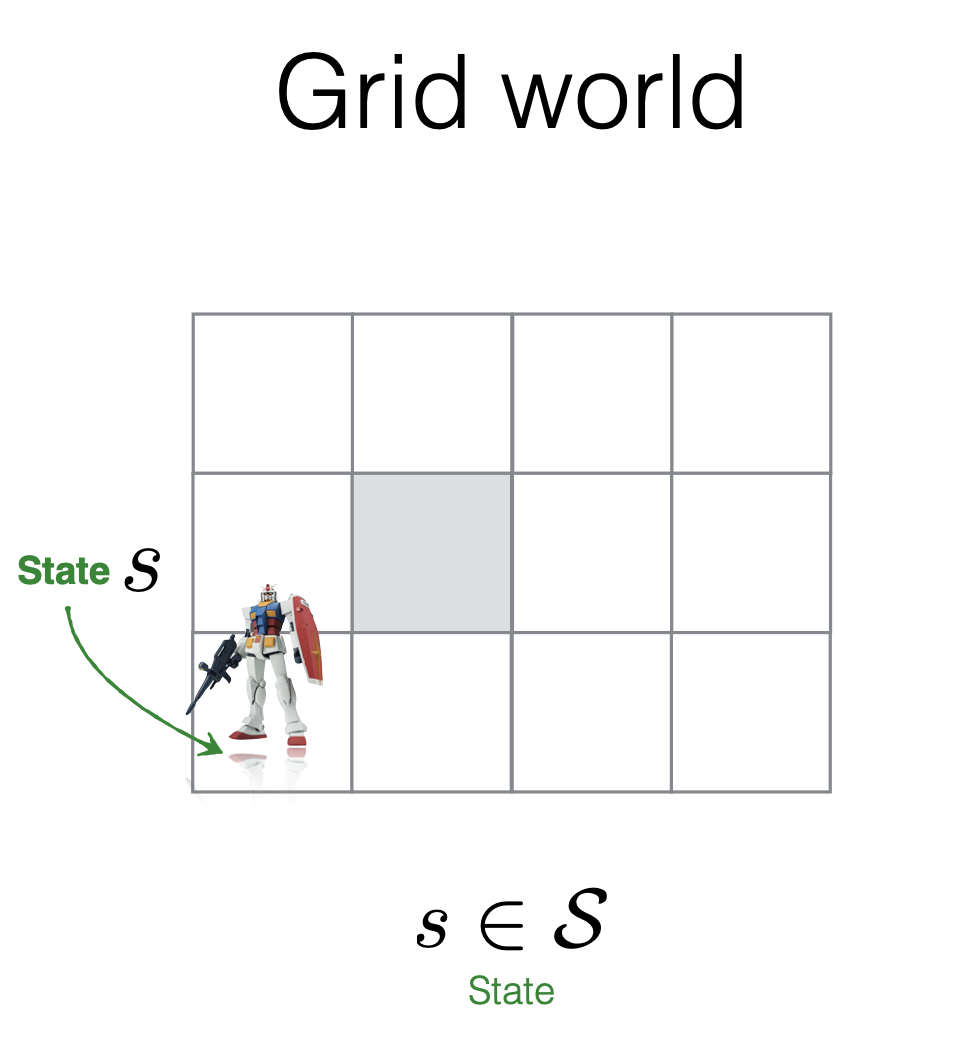
\includegraphics[width=\linewidth]{images/state.png}
     \end{subfigure}%
     \begin{subfigure}{0.3\linewidth}
         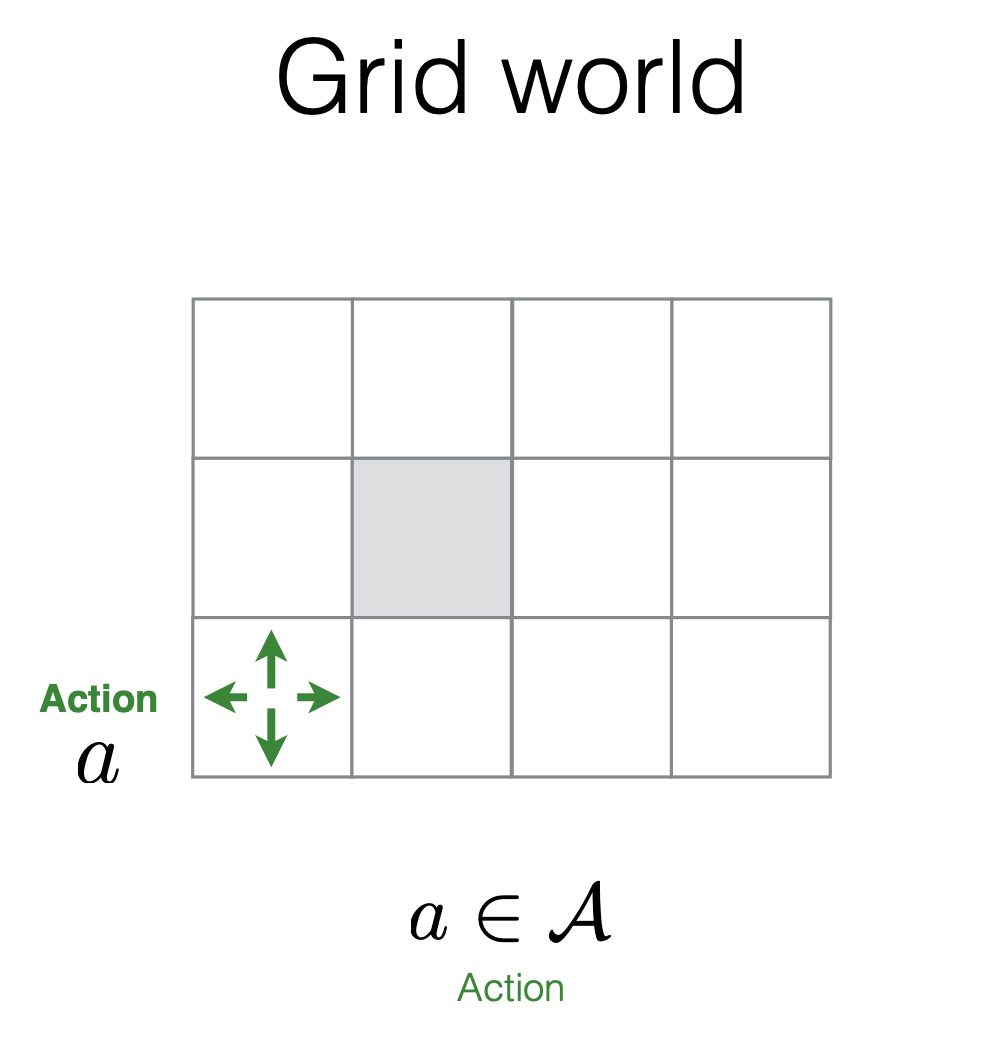
\includegraphics[width=\linewidth]{images/action.png}
     \end{subfigure}%
     \begin{subfigure}{0.3\linewidth}
         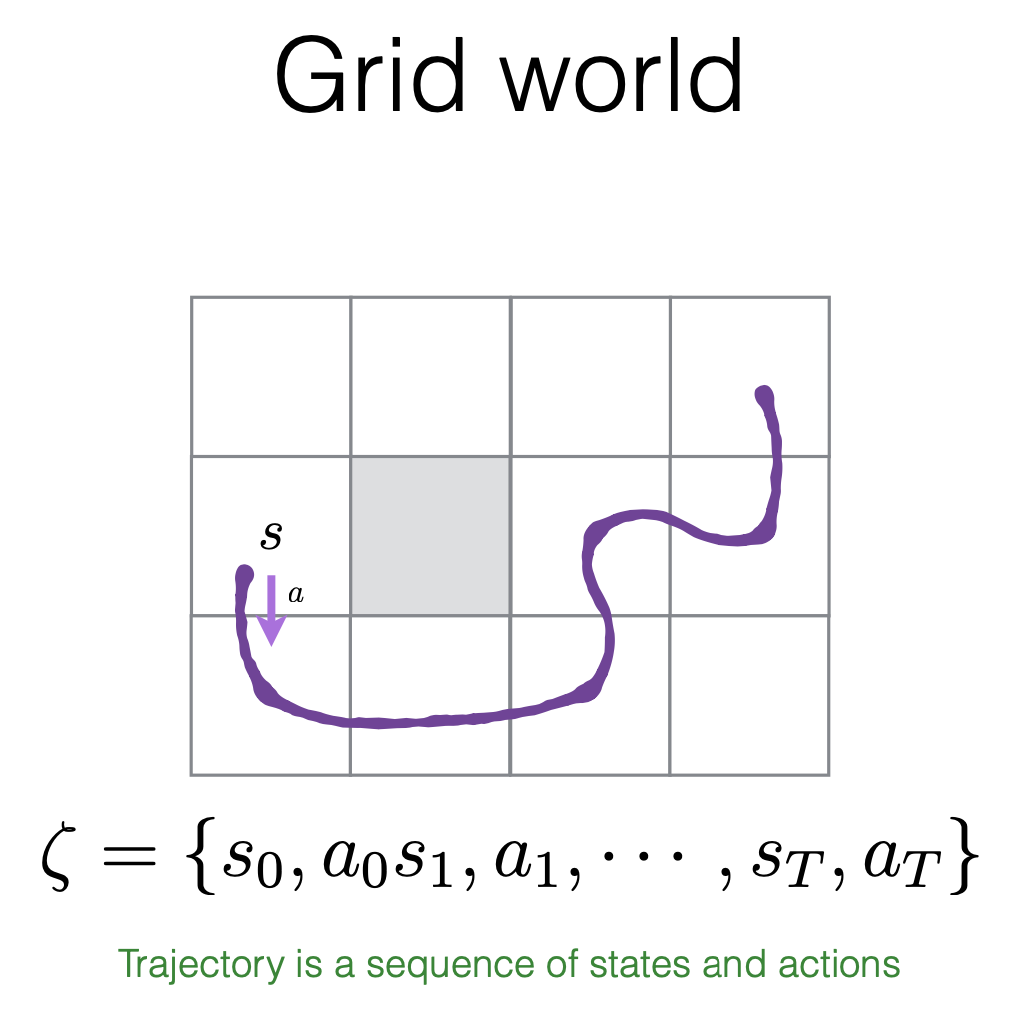
\includegraphics[width=\linewidth]{images/trajectory.png}
     \end{subfigure}%
    \label{fig:grid_world}
    \caption{State, action, and trajectory in a grid world.}
\end{figure}
In this grid world, each cell is a state, and the state is finite. There are actions you can take in each state. In this example, there are 4 actions: East, South, West and North. Trajectory is a sequence of states and actions.
Let's also look at some notations needed:
\begin{align*}
    & s \in \mathcal{S}  &\quad State \\
    & a \in \mathcal{A}  &\quad Action \\
    & p(s^{'} |s, a) &\quad State\; Transition\; Dynamic \\
    & r(s^{'} |s, a) &\quad Reward\; function \\
    & p_0(s) &\quad State\;prior \\
    & \pi (a|s) &\quad Policy \\
    & \gamma &\quad Discount\; factor
\end{align*}

\subsubsection{Setup of Markov Decision Process}

 MDP is way of sequential decision making and we can decompose it to a temporal sequence of variables. Let's define a trajectory as a sequence of states and actions $\zeta = \{s_0, a_0, s_1, a_1, ..., s_T, a_T\}$. Based on the trajectory, we consider the joint distribution of generating a trajectory $p(s_0, a_0, s_1, a_1, ..., s_T, a_T)$ and a reward function $r(s_0, a_0, s_1, a_1, ..., s_T, a_T)$, which is a scalar value for one trajectory. A traditional MDP factorization is as below:
 \begin{align*}
    p(s_0, a_0, ..., s_T, a_T) = p_0(s_0)\,\Pi_{t=0}^{T-1}\,p(s_{t+1}|s_t, a_t)p(a_t|s_t)
\end{align*}
The probability distribution over the whole trajectory can be decomposed to the prior state distribution $p_0$, which is the probability of a state you will start with, and a sequence product of state transition dynamic $p(s_{t+1}|s_t, a_t)$ and policy $p(a_t|s_t)$.
We call the reward function over the whole sequence return. There are also different factorization of the return.
\begin{align*}
    \textrm{Return} =  & r(s_0, a_0, s_1, a_1, ..., s_T, a_T) & \textrm{or} \\
      & r(s_0, a_0, s_1) + r(s_1, a_1, s_2) + ...  & \textrm{or}\\
      & r(s_0, a_0) + r(s_1, a_1) + ... & \textrm{or}\\
      & r(s_0) + r(s_1) + ...
\end{align*}
, where r(s) is the reward.

We can also look at it with a factor graphical model (Fig. \ref{fig:MDP_model}).
\begin{figure}[H]
    \centering
    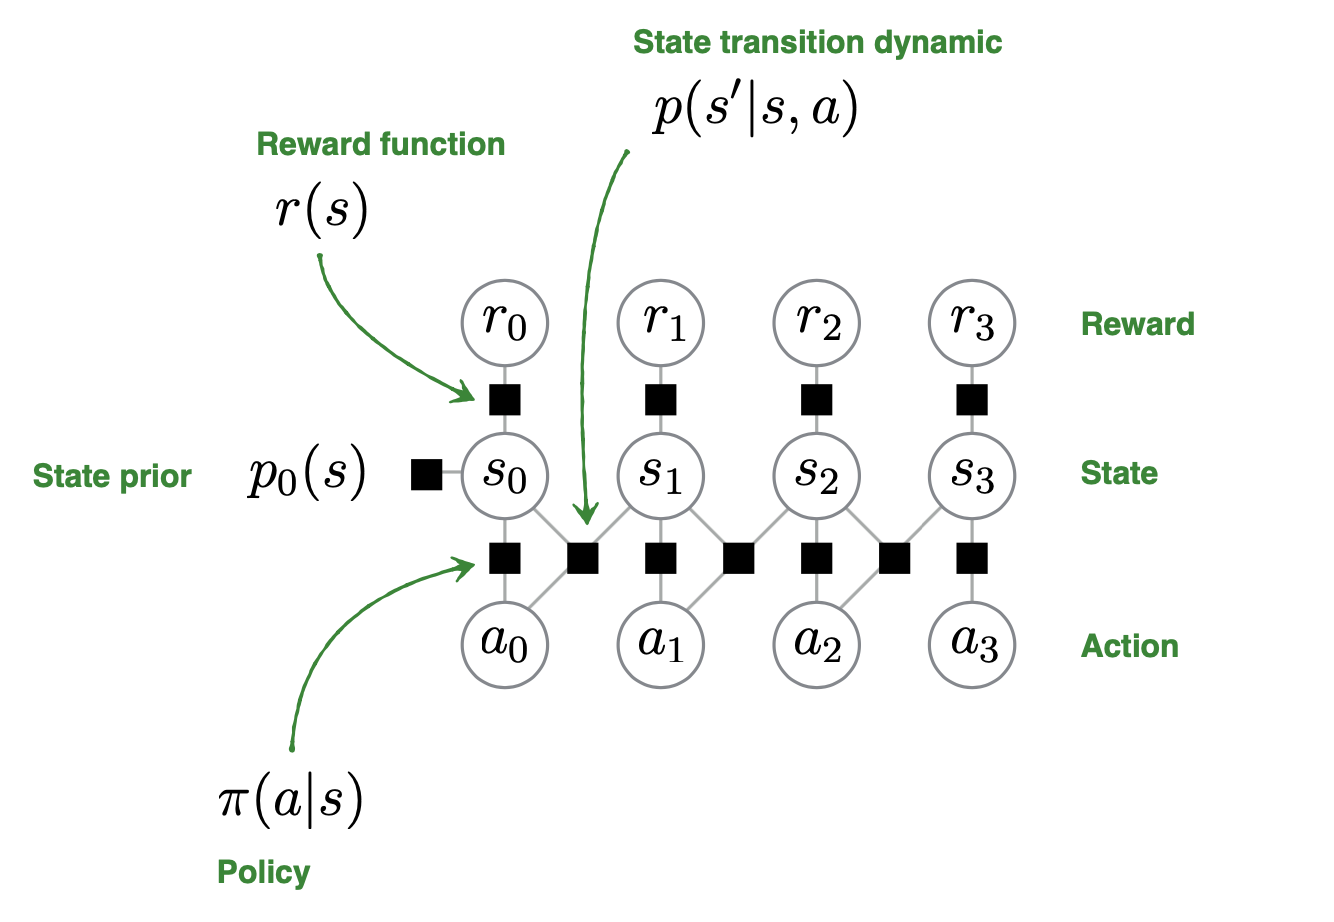
\includegraphics[width=.6\linewidth]{images/graphical_model.png}
    \caption{Graphical Model of MDP}
    \label{fig:MDP_model}
\end{figure}

Let's also describe the policy, state transition dynamic, and reward in the grid world (Fig.~\ref{fig:grid_world_policy}). Policy describes which action to take in a given state. State transition dynamic describes the probability of transition to another state. Reward function maps a state to a real value; in this example, we have the reward value finite.
\begin{figure}[H]
    \centering
     \begin{subfigure}{0.3\linewidth}
         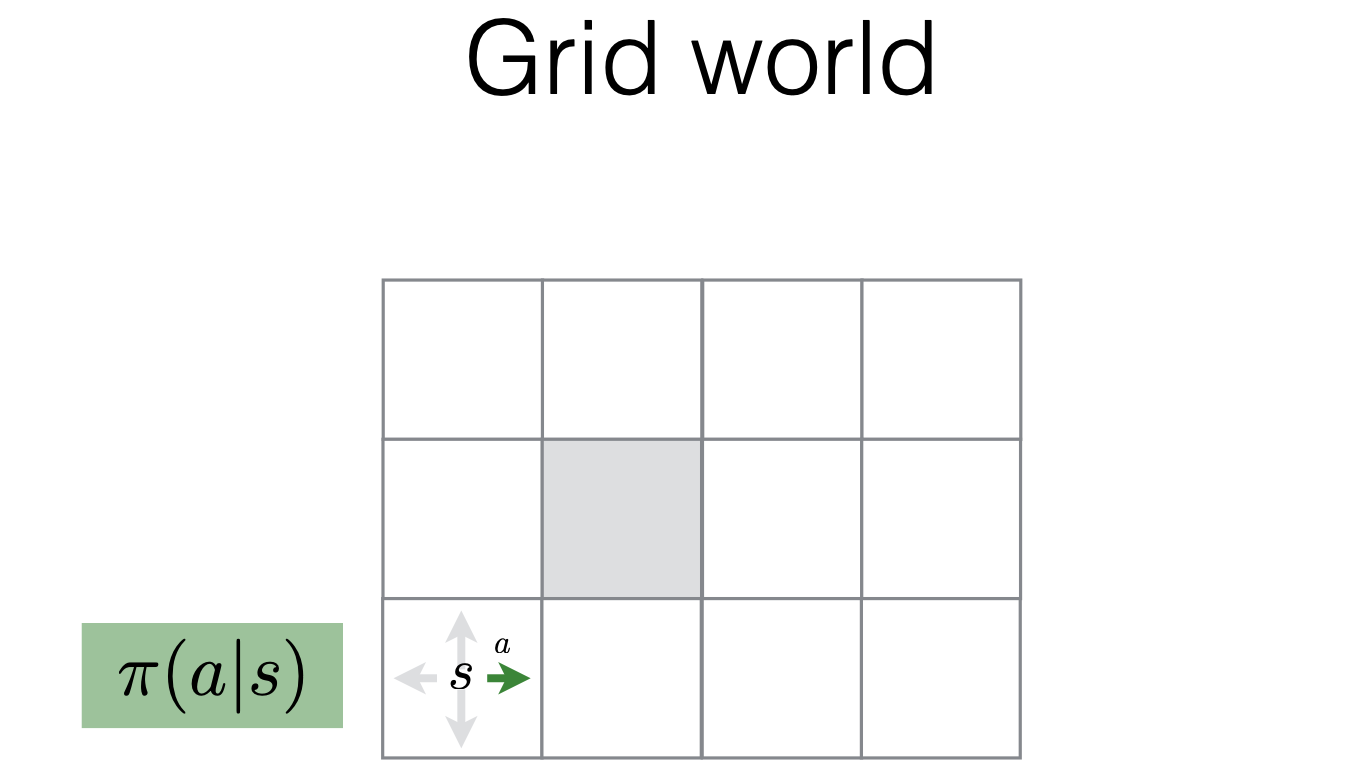
\includegraphics[width=\linewidth]{images/policy.png}
     \end{subfigure}%
     \begin{subfigure}{0.3\linewidth}
         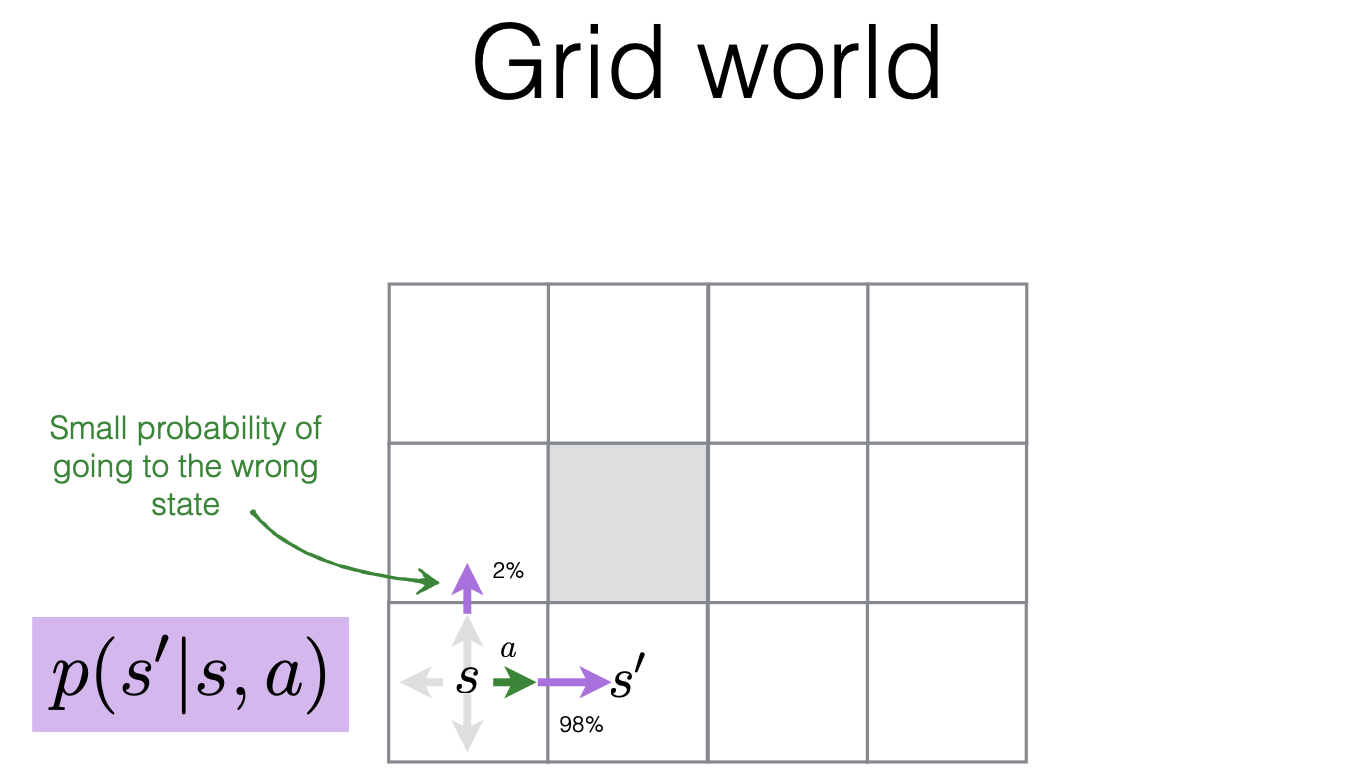
\includegraphics[width=\linewidth]{images/state_transition.png}
     \end{subfigure}%
     \begin{subfigure}{0.3\linewidth}
         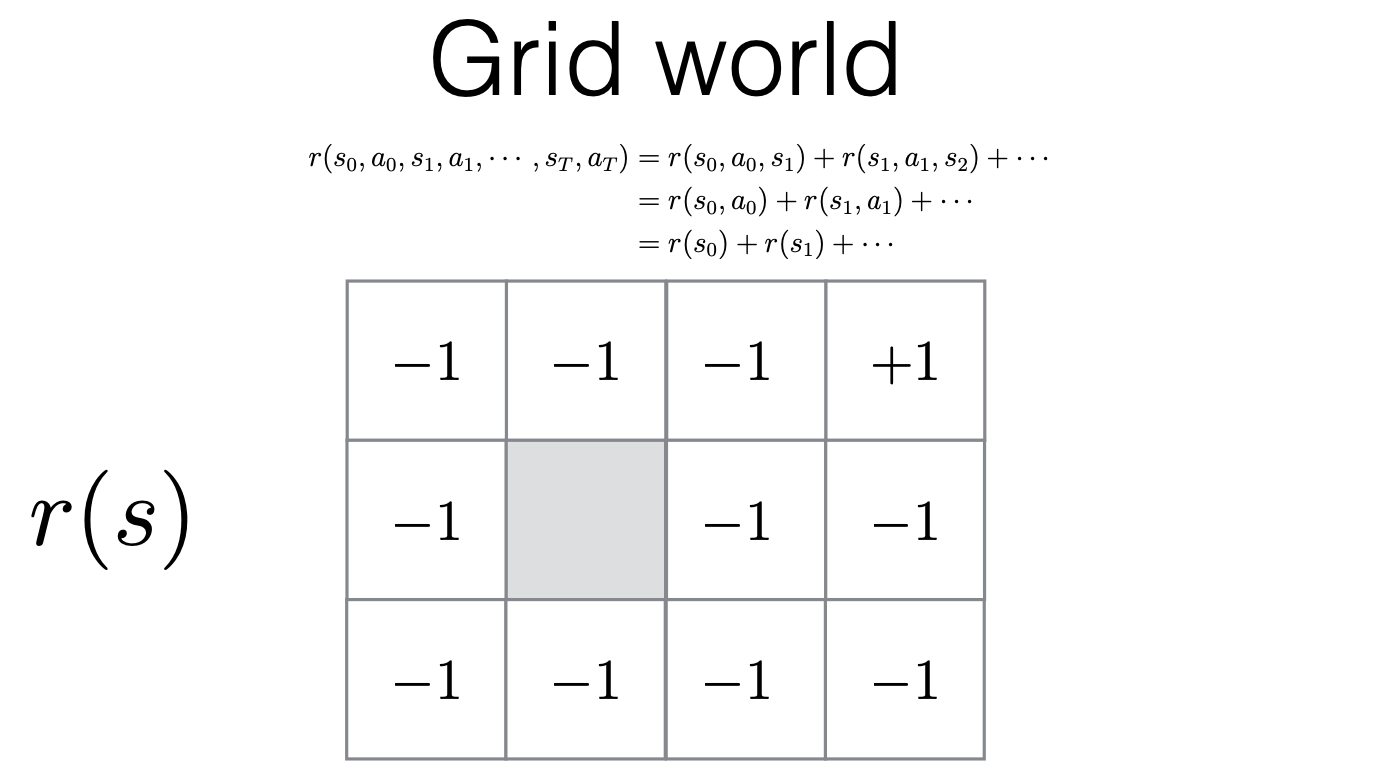
\includegraphics[width=\linewidth]{images/reward.png}
     \end{subfigure}%
    \caption{Policy, state transition dynamic, and reward in a grid world.}
    \label{fig:grid_world_policy}
\end{figure}

There are many inference tasks for the MDP. Fig.\ref{fig:MDP_tasks} visualize the problems to solve for. Reinforcement learning, where we target at solving for policy, and inverse reinforcement learning, where we target at solving for reward function will be covered in class.

\begin{figure}[H]
    \centering
    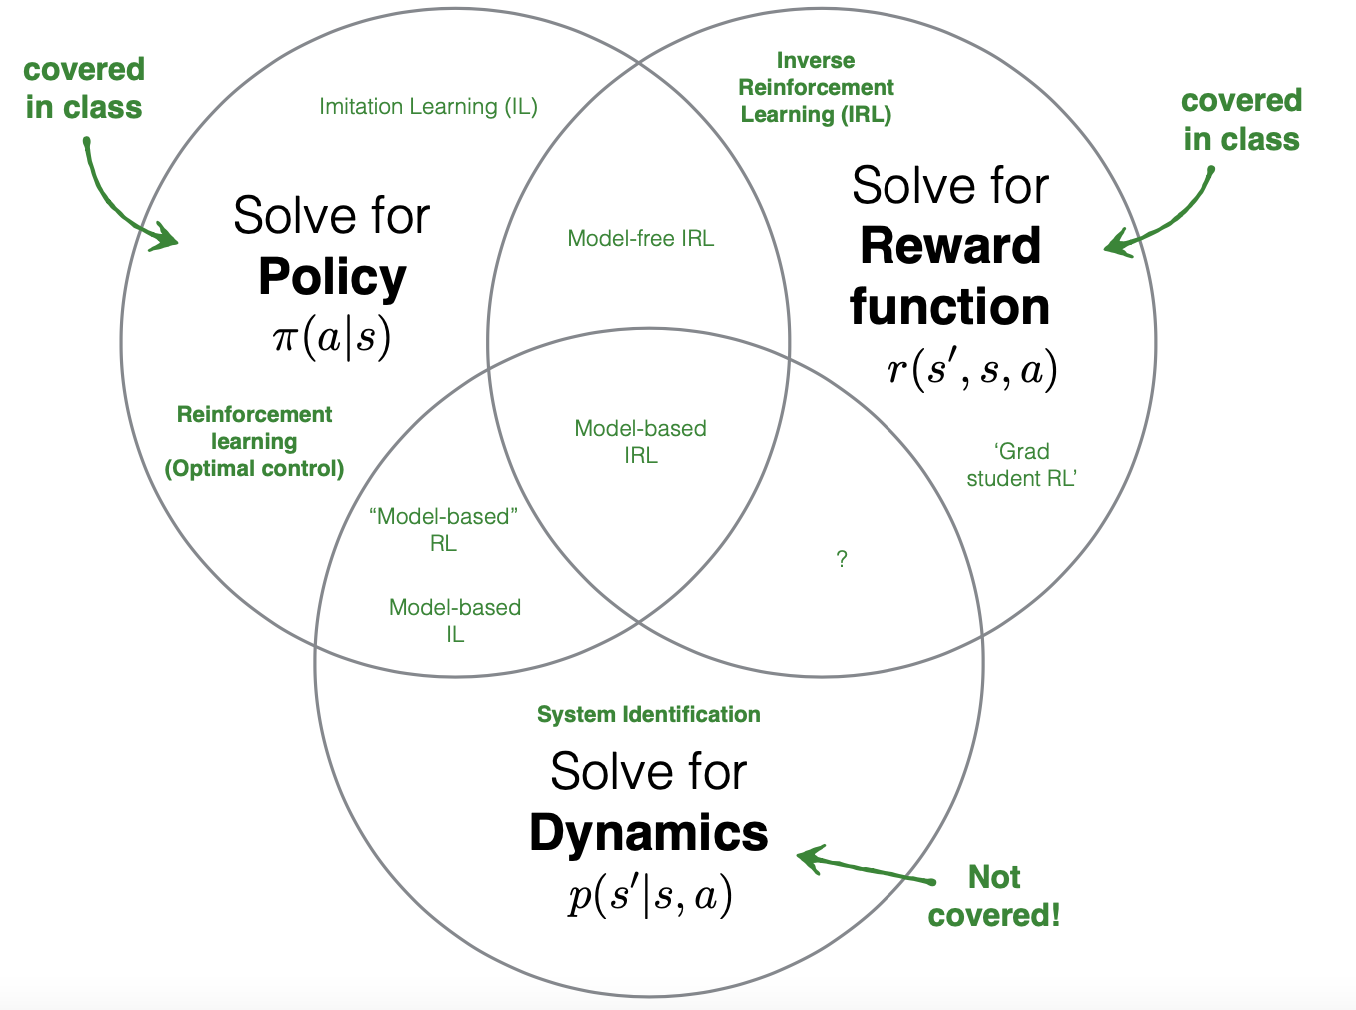
\includegraphics[width=.45\linewidth]{images/MDP_tasks.png}
    \caption{Inference tasks of MDP}
    \label{fig:MDP_tasks}
\end{figure}
There are many RL approaches to find the optimal policy. We can divide it into policy-based, valued-based, and hybrid. There are also many assumptions when finding the optimal policy. Two big categories are:
\begin{itemize}
    \item Model-based
    \begin{itemize}
        \item Dynamics known
        \item Reward function known
    \end{itemize}
    \item Model-free
    \begin{itemize}
        \item Dynamics unknown
        \item Reward function unknown
        \item Learn through interaction
    \end{itemize}
\end{itemize}

\subsubsection{MDP Concepts}
\textbf{Value Function}
Value function is to predict the future. A type of value functions is \emph{state value function}, which only depends on states. It is the total expected return of a trajectory in a state s.
\begin{align*}
    V^{\pi}(s) = \mathbb{E}_p[r_0 + r_1 + r_2 + ... | s_0 = s]
\end{align*}
, where $r_t \triangleq r(s_{t+1}=s^{'}, a_t=a, s_t=s)$ and p is the joint distribution of the MDP. Since it i shard to deal with infinite return, we usually have \emph{finite horizon return} and \emph{infinite horizon discounted return}:
\begin{align*}
    V^{\pi}(s) = \mathbb{E}_p[r_0 + r_1 + r_2 + ... + r_T| s_0 = s] \\
    V^{\pi}(s) = \mathbb{E}_p[\gamma^0 r_0 + \gamma^1 r_1 + \gamma^2 r_2 + ... | s_0 = s]
\end{align*}

Another type of value function is \emph{state-action value function}. It is the total expected return of a trajectory starting in state s and taking action a.
\begin{align*}
    Q^{\pi}(s, a) = \mathbb{E}_p[\gamma^0 r_0(s_0) + \gamma^1 r_1(s_1) + \gamma^2 r_2(s_2) + ... | s_0 = s, a_0 = a]
\end{align*}
The relationship between $V$ and $Q$ is
\begin{align*}
    V^{\pi} = \sum_a\pi(a|s)Q^\pi(s, a)
\end{align*}
We use the value function to be the objective function of RL. In other words, we want to find the best policy by maximizing the value function.
\begin{align*}
    \hat{\pi} & = \argmax{\pi} V^{\pi}(s) \\
    & = \argmax{\pi} \mathbb{E}_p[\sum_{t=0}^{\infinity} \gamma^t r_t | s_0 = s]
\end{align*}

%\section*{References}
%Include your references here. Please cite any resources you found useful.	
%Populate the refs.bib file or list your references manually. Be consistent in formatting!
{
\bibliography{refs}
\bibliographystyle{abbrv}
}

%\section{Appendix}
%This section provides any relevant background material that was not covered in the lectures, but was found to be useful for understanding the material. 
%For example, derivations, theory underlying techniques employed, etc. 

%Additionally, this section can summarizes applications or extensions of these techniques found in the literature. 

\end{document} % Done!


